
\begin{figure}[t]
    \begin{centering}
        % \subfloat[Some cool graphic]
        {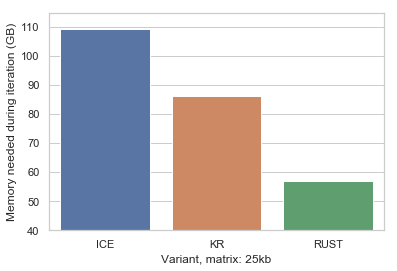
\includegraphics[scale=1]{figures/results/memiter_25}}
        \caption[Memory needs iterating 25kb]
        {\textbf{Memory needed during iteration} for correcting the 25kb matrix. Smaller is better.}
        \label{fig:memiter25}
\end{centering}
\end{figure}

\begin{figure}[t]
    \begin{centering}
        \subfloat[Available data]
        {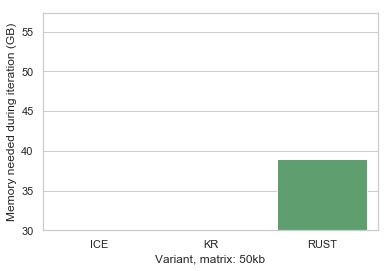
\includegraphics[scale=0.5]{figures/results/memiter_50}}
        \subfloat[Extrapolated data]
        {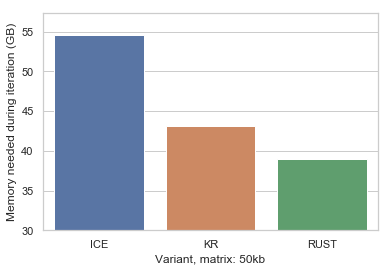
\includegraphics[scale=0.5]{figures/results/memiter_50_extra}}
        \caption[Memory needs iterating 50kb]
        {\textbf{Available and Extrapolated Data about Memory needed during
        iteration} of the 50kb matrix. Rust value is accurate, values for ICE
        and KR are not accurately available, but have been observed to be in
        the extrapolated areas. Smaller is better.}
        \label{fig:memiter50}
    \end{centering}
\end{figure}




\begin{figure}[t]
    \begin{centering}
        \subfloat[Maximum resident set size when correcting 50kb matrix]
        {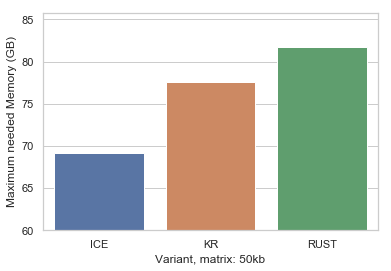
\includegraphics[scale=0.9]{figures/results/maxresident_50}} \\
        % \caption[Maximum needed Memory for 50kb]
        % {\textbf{Maximum needed Memory} when correcting the 50kb matrix.}
        \subfloat[Maximum resident set size when correcting 25kb matrix]
        {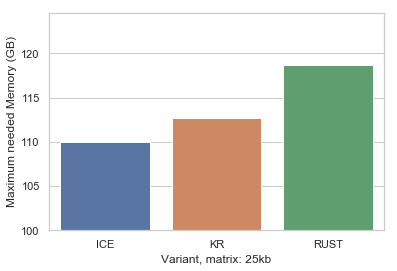
\includegraphics[scale=0.9]{figures/results/maxresident_25}}
        \caption[Maximum needed Memory]
        {\textbf{Maximum amount of needed Memory} when correcting 50kb and 25kb
        matrix. Note that the Python ICE values are likely inaccurate. Smaller is better.}
        \label{fig:maxresident}
    \end{centering}
\end{figure}


\begin{figure}[t]
\begin{centering}
    \subfloat[Runtime in minutes for correcting 25kb Matrix]
    {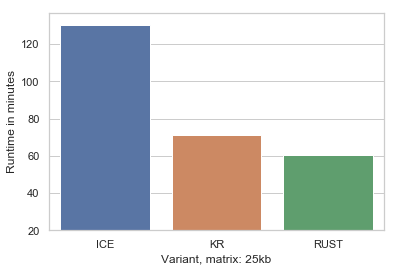
\includegraphics[scale=0.9]{figures/results/runtime_25}} \\
    % \caption[Correction time of 25kb]
    % {\textbf{Runtime in minutes} for correcting the 25kb matrix.}
    \subfloat[Runtime in minutes for correcting 50kb Matrix]
    {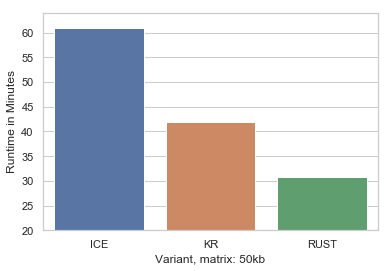
\includegraphics[scale=0.9]{figures/results/runtime_50}}
    \caption[Algorithm Runtimes]
    {\textbf{Algorithm Runtimes} for correcting the different matrices. Smaller is better.}
    \label{fig:runtime}
\end{centering}
\end{figure}

\begin{figure}[t]
    \begin{centering}
        \subfloat[Loading time in minutes for 25kb matrix]
        {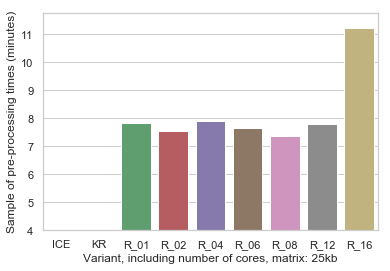
\includegraphics[scale=0.9]{figures/results/loadtimes_25}} \\
        % \caption[Correction time of 25kb]
        % {\textbf{Runtime in minutes} for correcting the 25kb matrix.}
        \subfloat[Loading time in minutes for 50kb matrix]
        {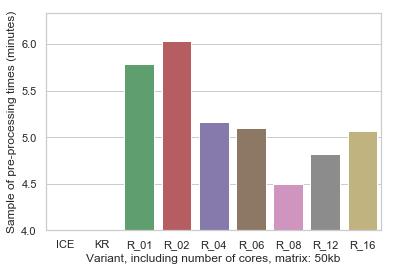
\includegraphics[scale=0.9]{figures/results/loadtimes_50}}
        \caption[Matrix loading times]
        {\textbf{Matrix loading times} for the different matrix sizes. Even though
        the operations are the same during pre-processing, actual times fluctuated
        somewhat. No data is available for ICE and KR variants, however as the
        pre-processing is the same, their values can be thought to be in the same
        range as the others.
        Equal is better.}
    \label{fig:loadtimes}
\end{centering}
\end{figure}



